\documentclass[sigconf, screen, review]{acmart}

%% The Web Conference 2027 - Demo Track
%% Max 4 pages including references. Submission: OpenReview, 16 Nov 2026 (AoE).
%% TODO before submission:
%%   1. Record the 2-minute screencast and replace TODO_VIDEO below.
%%   2. Figure 2 is cut from paper/fig-demo.png (store, reply and terminal regions).
%%   3. Confirm the venue notice promised in the ethics section.

\usepackage{tikz}
\usetikzlibrary{calc}

\setcopyright{none}
\settopmatter{printacmref=false}
\renewcommand\footnotetextcopyrightpermission[1]{}
\pagestyle{plain}
\acmConference[WWW '27]{The ACM Web Conference 2027}{May 10--14, 2027}{Dublin, Ireland}

\begin{document}

\title{Silicon Shoppers: An Adaptive Storefront the Shopper Can Operate}

\author{Prabhu Pugalenthi}
\affiliation{%
  \institution{University of Southern California}
  \city{Los Angeles}
  \state{CA}
  \country{USA}}
\email{pugalent@usc.edu}

\author{Ansel Zeng}
\affiliation{%
  \institution{University of Southern California}
  \city{Los Angeles}
  \state{CA}
  \country{USA}}
\email{anselzen@usc.edu}

\author{Sumin Jo}
\affiliation{%
  \institution{University of Southern California}
  \city{Los Angeles}
  \state{CA}
  \country{USA}}
\email{suminjo@usc.edu}

\begin{abstract}
E-commerce personalization stops at the recommendation rail: the store itself looks identical for every shopper, and when the underlying model is wrong the shopper has no recourse. We present \emph{Silicon Shoppers}, a deployed web storefront in which the entire layout (navigation order, hero advertisements, homepage rails, listing sort, filters, badges, and checkout variant) is a typed, versioned document that three different writers can mutate: a purchase-history model, a live browsing model, and the shopper, speaking to an LLM concierge. The concierge is not decorative: it emits structured actions that are validated, executed, and audited against real store state, so a reply that claims an action the model did not emit is either recovered into a real state change or honestly corrected. A staged animation engine plays every layout change component by component, making the rearrangement itself inspectable. Attendees can chat with the concierge, rearrange the store in natural language, complete a purchase end to end, and watch every model decision, layout step, and agent action narrated live on a companion terminal.
\end{abstract}

\begin{CCSXML}
<ccs2012>
<concept>
<concept_id>10002951.10003317.10003331</concept_id>
<concept_desc>Information systems~Users and interactive retrieval</concept_desc>
<concept_significance>500</concept_significance>
</concept>
<concept>
<concept_id>10002951.10003317.10003347.10003350</concept_id>
<concept_desc>Information systems~Recommender systems</concept_desc>
<concept_significance>300</concept_significance>
</concept>
<concept>
<concept_id>10003120.10003121.10003129</concept_id>
<concept_desc>Human-centered computing~Interactive systems and tools</concept_desc>
<concept_significance>300</concept_significance>
</concept>
</ccs2012>
\end{CCSXML}

\ccsdesc[500]{Information systems~Users and interactive retrieval}
\ccsdesc[300]{Information systems~Recommender systems}
\ccsdesc[300]{Human-centered computing~Interactive systems and tools}

\keywords{personalization, LLM agents, conversational commerce, adaptive interfaces, tool-use faithfulness}

\maketitle

% ============================================================
\section{Introduction}

Online personalization has converged on a single shape: a fixed storefront with a recommendation shelf stapled on. The navigation, the hero banner, the order of homepage sections, the sort order of a listing, the structure of the store, is identical for a first-time browser and a decade-long customer. Meanwhile, a new generation of LLM agents is being deployed into consumer settings, where they do more than answer questions: they add items to carts, apply filters, and initiate payments. Two problems meet here. First, shoppers cannot talk back to the store; the model's decisions are opaque and unappealable. Second, LLM agents that act remain unreliable on realistic multi-step tasks \cite{taubench, webarena}, and they are unreliable narrators of their own behavior: in development our concierge repeatedly reported actions it had never executed.

Silicon Shoppers is a personalization engine, demonstrated inside a fashion storefront we built (SoCal Atelier), around a simple idea: the store layout itself is data, and an agent can act on it. Three writers mutate one typed, versioned layout contract: (i) a model trained on purchase history merchandises the store before first paint, and a warehouse job rescores the shopper every four minutes; (ii) in-session models adapt the store on every click; and (iii) the shopper, through a concierge chat, rearranges the store in natural language (``make this more men-friendly, navy forward'') or delegates whole tasks to it (``buy the wool trouser in black, size M''). Every change plays as a staged animation, and every model input, layout output, and event persists to Snowflake.

The demo's technical contribution is the agent's \emph{honesty layer}: a pipeline in which the agent's actions are validated against the real catalog before it writes its reply, recovered from claim prose when absent, and audited against actual state transitions before any claim reaches the shopper.

\textbf{Related work.} Adaptive interfaces have a long history, from decision-theoretic interface generation \cite{supple} to whole-page presentation learned for search results \cite{wholepage}; there the system alone chooses the layout. Agent benchmarks \cite{taubench, webarena, workarena, osworld} score task success after the fact in sandboxes, and work on tool use \cite{react, gorilla, toolllm} improves how reliably a model selects and calls an API. Silicon Shoppers differs on both counts: the shopper edits the same layout object the models write, and the agent's claims are checked against store state at run time, inside a consumer interface.

% ============================================================
\section{System Overview}

Figure~\ref{fig:arch} shows the architecture. The system has three surfaces (the storefront, a simulator shell that hosts and instruments it, shown in Figure~\ref{fig:demo}, and a data plane that persists everything) connected by a single typed layout contract.

\begin{figure*}[t]
  \centering
  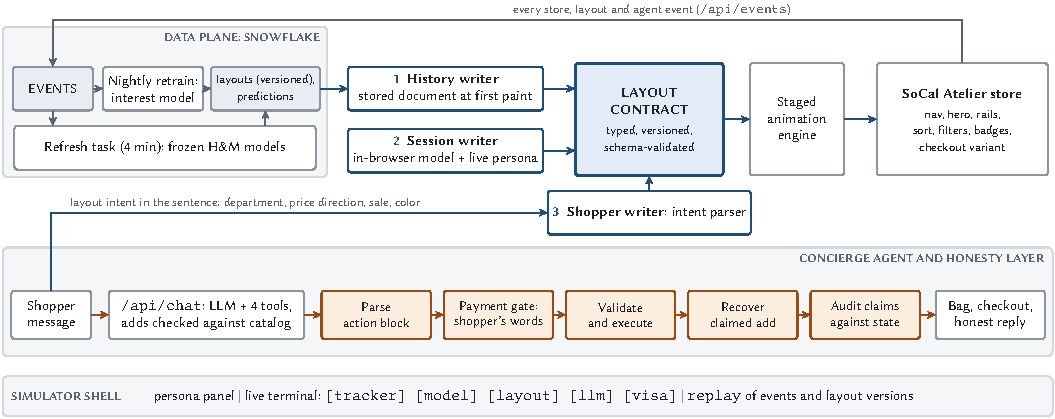
\includegraphics[width=0.9\textwidth]{figures/architecture.pdf}
  \caption{Silicon Shoppers architecture. Three writers mutate one layout contract (blue): (1) the stored document, recomputed every four minutes with the frozen purchase models; (2) the in-browser session model and live persona; (3) the shopper, through a deterministic intent parser. Concierge replies pass through the honesty layer (orange) before they reach the bag or the shopper.}
  \label{fig:arch}
  \Description{Block diagram. A Snowflake data plane holds store events, a refresh task that runs every four minutes, stored layouts, and a nightly retrain. Three writers (history, session, shopper) feed a central layout contract, which feeds a staged animation engine and then the store. Below, a shopper message flows through the chat endpoint with an LLM and four tools, then through five honesty stages (parse, payment gate, validate and execute, recover, audit) to the bag, checkout, and reply. A simulator shell with a persona panel, live terminal, and replay observes everything.}
\end{figure*}

\subsection{The layout contract}

The contract, \texttt{atelier.store\_layout.v1}, is one versioned JSON document per shopper with 22 layout decisions: department and category order, homepage sections, hero, default sort, filter order, color highlight, badges, pop-ups, grid density, comparison and quick-add UI, and checkout variant. Each decision records its value, whether it departs from the default store, a human-readable reason, and its source. The store turns the document into what it renders (navigation, ad placements, homepage blocks, listing sort and filters, cards, checkout) through one validator that repairs small problems, reports each fix, and falls back to the default store when a configuration cannot be parsed, so no writer, model or human, can produce a malformed store. Because layout is data rather than code, it can be diffed, replayed, audited, and animated. All three writers mutate the same contract, which is what makes shopper control a feature of the store itself rather than a settings page. The shell can also ask an LLM to design within the same schema; the validator keeps the model's confirmed orderings and drops any LLM-written reason that cites a number absent from the model output.

\subsection{Two personalization models}

\textbf{First paint.} Purchase models trained on 100,000 shoppers from the H\&M Personalized Fashion Recommendations dataset \cite{hmdataset} predict a shopper's mix over departments, categories, sections, and colors for the next four weeks. Each layout decision follows from that prediction and carries its reason (``Sale first: about 41\% of your next picks'') and a flag saying whether that decision type was confirmed on held-out purchases. On a reserved 2019 window with 100,000 shoppers outside the training cohort (15,035 buyers), scored once after the models were frozen, personalized section order improved NDCG over the default store by 0.020 (95\% CI 0.018 to 0.021) and the color highlight raised the share of next purchases in the highlighted colors by 0.047 (0.039 to 0.056); category order was not confirmed and is flagged as such. A store shopper is scored by mapping bag adds onto H\&M product groups and colors, a mapping that is itself untested. Each document also names a descriptive persona (\emph{Price Hunter}, \emph{Trend Seeker}, \emph{Mission Shopper}, or \emph{Brand Loyalist}) scored from interpretable signals (markdown affinity, novelty affinity, purchase frequency, category concentration, rebuy share). At medium confidence or above the persona overlays the layout: a Price Hunter sees sale-forward navigation and price-ascending sort.

\begin{figure*}[t]
  \centering
  % Three regions cut from one screenshot of the running app (figures/capture_demo.py).
  % Callout positions are fractions of the store image: (x from left, y from top).
  \newcommand{\storew}{3.340in}
  \newcommand{\storeh}{2.085in}
  \newcommand{\sidew}{3.095in}
  \newcommand{\callout}[3]{\node[circle, fill={rgb,255:red,31;green,78;blue,121}, draw=white, line width=.6pt,
    text=white, inner sep=1.1pt, font=\sffamily\bfseries\fontsize{6.5}{6.5}\selectfont]
    at (#1*\storew, -#2*\storeh) {#3};}
  \begin{tikzpicture}[inner sep=0pt]
    \node[anchor=north west] (store) at (0,0) {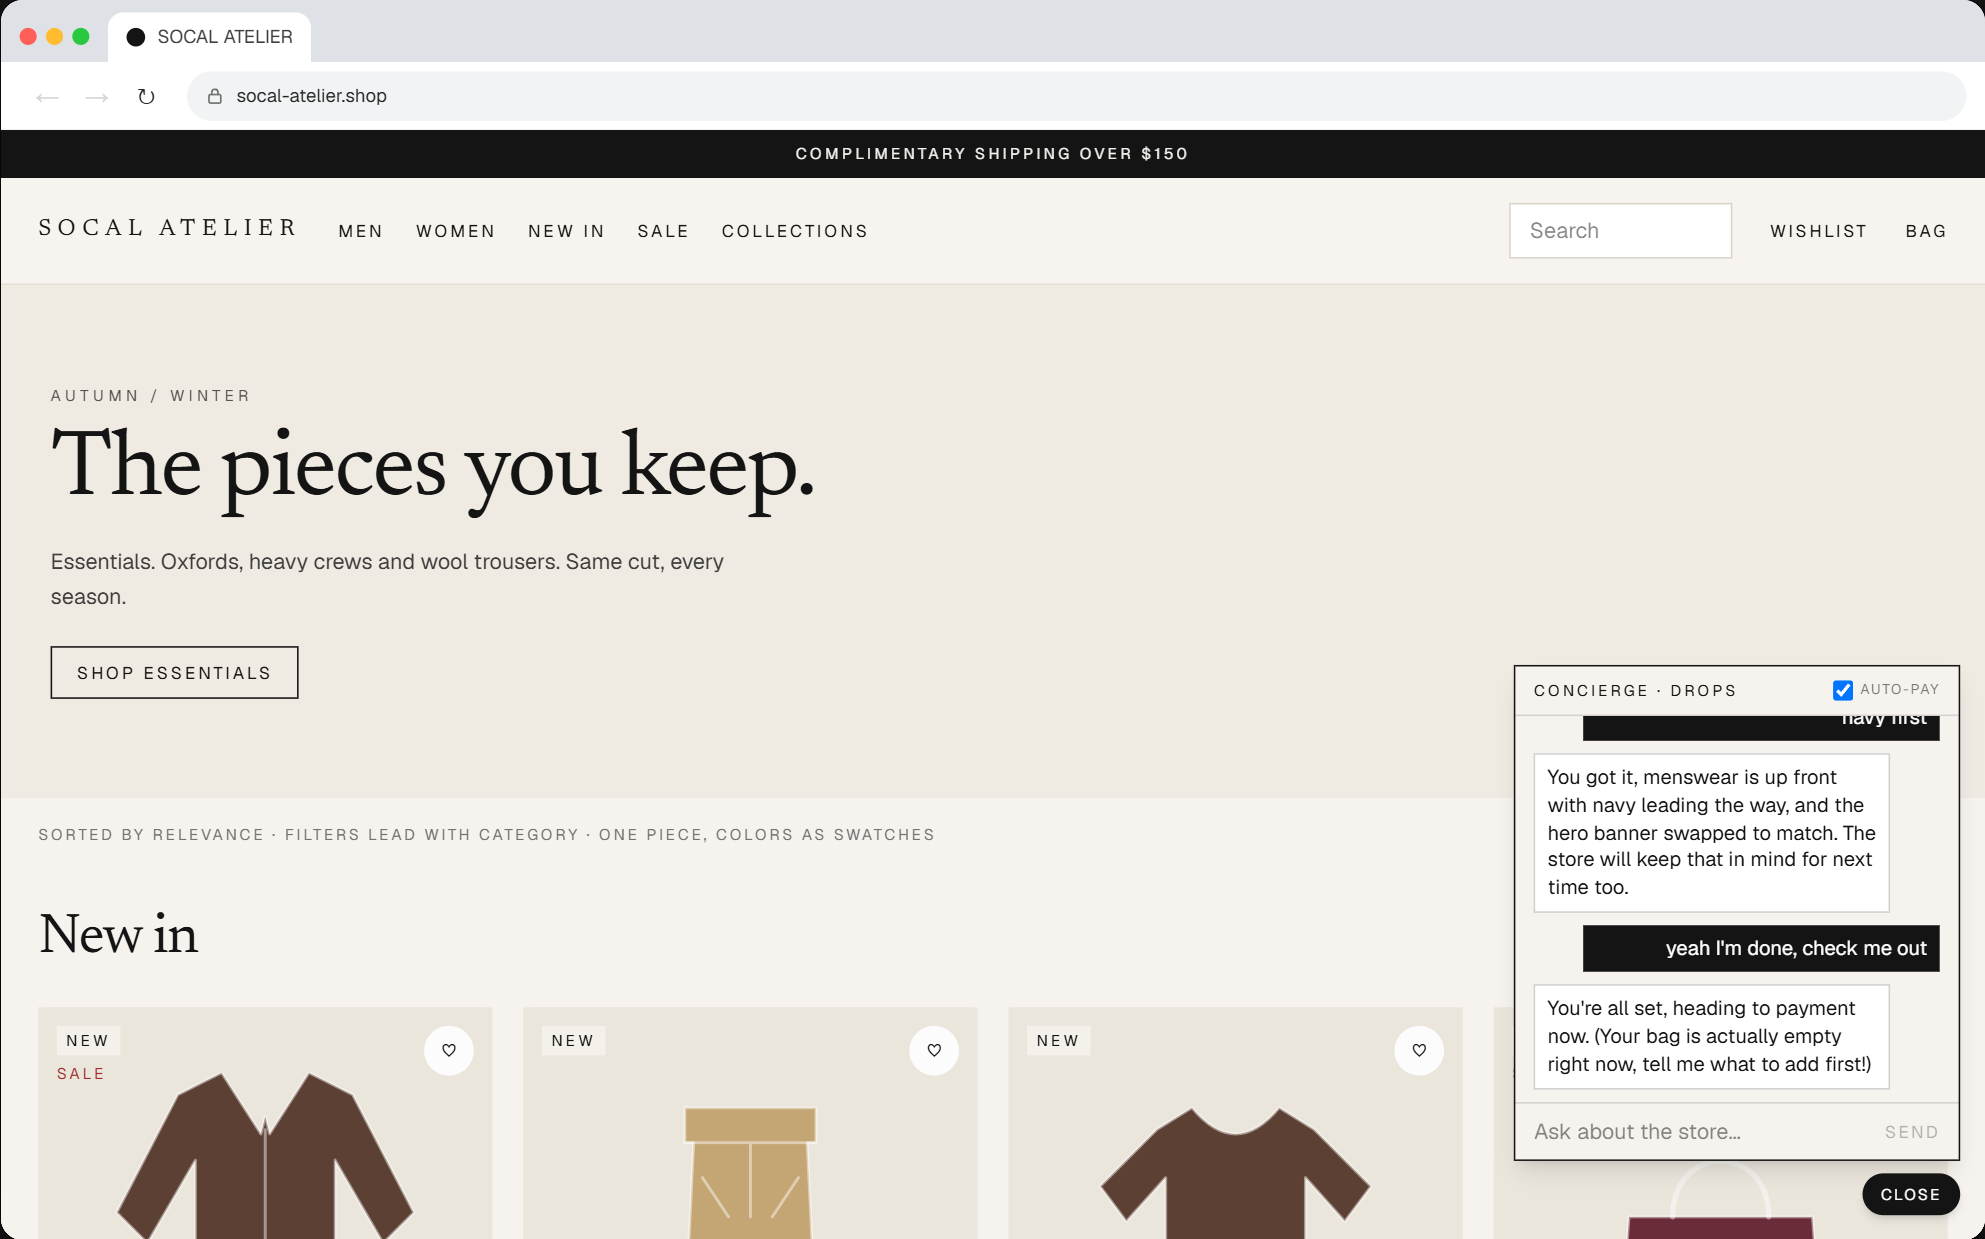
\includegraphics[width=\storew]{figures/demo-store.png}};
    \node[anchor=north west] (reply) at ($(store.north east)+(0.08in,0)$) {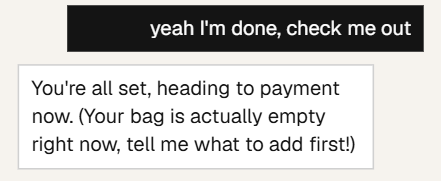
\includegraphics[width=\sidew]{figures/demo-reply.png}};
    \node[anchor=south west] (term) at ($(store.south east)+(0.08in,0)$) {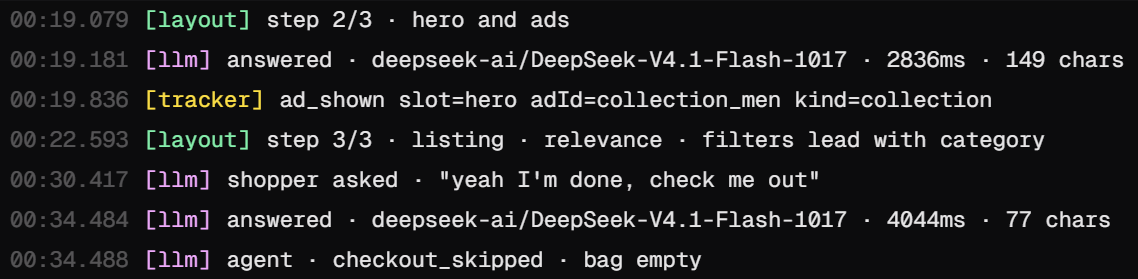
\includegraphics[width=\sidew]{figures/demo-terminal.png}};
    \callout{0.181}{0.228}{1}
    \callout{0.435}{0.375}{2}
    \callout{0.745}{0.535}{3}
  \end{tikzpicture}
  \caption{The store and terminal after two concierge turns (regions of one screenshot). The first sentence moved menswear to the front of the navigation (1) and swapped the hero (2). The second (3, enlarged at right) asked to pay with an empty bag: with tools off the model announced payment, and the audit appended the correction in parentheses; the terminal shows the skipped checkout.}
  \label{fig:demo}
  \Description{Screenshot of the demo. On the left, the SoCal Atelier store in a browser frame shows Men first in the navigation, a hero reading The pieces you keep, and the open concierge chat. On the top right, an enlarged part of the chat shows the shopper's message, yeah I'm done, check me out, and the reply, You're all set, heading to payment now, followed in parentheses by, Your bag is actually empty right now, tell me what to add first. On the bottom right, a terminal lists layout steps, two model replies with their latency, and an agent line reading checkout skipped, bag empty.}
\end{figure*}

\textbf{In-session.} Two components adapt the store while the shopper browses. A LightGBM session model trained on the OTTO dataset \cite{otto} sees only the first 3 to 40 events of a session and predicts browsing style over the rest of it. It runs in the browser and re-derives per-field browsing decisions (grid density, comparison UI, quick-add, product-page density) after every click; a field activates only once held-out $R^2$ for every style value behind it, at that many events, reaches 0.10 (Figure~\ref{fig:r2}). Alongside it, a provisional persona is computed live from the shopper's own event stream (sale adds, price sorts, newest sorts, filters, searches, repeat views), nudged by the OTTO model's predicted browsing style. The persona is named only once enough evidence exists (at least five events and a minimum score), and only at medium confidence may it touch the layout, reordering navigation, hero, rails, and sort. Once the refresh loop has stored a persona scored on the shopper's whole history, that one takes over, so the panel, the terminal, the layout, and the concierge always name the same persona. Every applied decision carries a reason string the UI surfaces on demand (``why am I seeing this?'').

\begin{figure}[t]
  \centering
  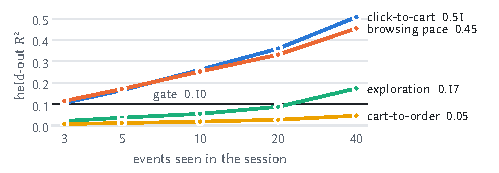
\includegraphics[width=\columnwidth]{figures/session-r2.pdf}
  \caption{Held-out $R^2$ of the session model on single-visit OTTO prefixes (four of seven style values). A decision switches on only when every value behind it clears the gate; cart reminders, which need cart-to-order, stay off within one visit.}
  \label{fig:r2}
  \Description{Line chart. Horizontal axis: events seen in the session, 3 to 40. Vertical axis: held-out R squared, 0 to 0.5. Click-to-cart rises from 0.11 to 0.51 and browsing pace from 0.11 to 0.45, both above the 0.10 gate throughout. Exploration rises from 0.02 to 0.17 and crosses the gate only at 40 events. Cart-to-order stays below 0.05.}
\end{figure}

\subsection{The concierge agent}

The chat bubble streams responses from DeepSeek-V4.1-Flash via the Nebius API (Gemini is a drop-in alternative) through an NDJSON endpoint. Each request carries a grounded context payload (persona, decision reasons, bag contents, and what the shopper has told the concierge before), so questions like ``why am I seeing this?'' are answered from data.

The agent looks things up and acts through four server-side tools: \texttt{search\_products}, \texttt{check\_bag}, \texttt{add\_to\_bag}, and \texttt{checkout}. Products reach the model only as tool results from the full catalog, and an add is checked (product, color, size) before the model writes its reply; a refused add comes back with the reason and real alternatives. Because the bag lives in the browser, validated calls are handed to it as a typed action block, which the reply handler executes under the guards below. A provider without tool calling writes that block itself from a catalog in the prompt. Layout intent in the shopper's message (department, price direction, sale negation, color focus) is mapped onto contract edits by a deterministic parser and plays through the same staged animation as model-driven changes. The sentence is stored with the event and re-applied on later visits until the shopper asks the concierge to forget it.


\subsection{The honesty layer}

Deployed shopping agents fail in a specific way we observed repeatedly in development: the model claims an action it never performed. Our defense is layered, and each layer is independently testable:

\begin{enumerate}
  \item \textbf{Prompt.} Claims must be backed by a tool call; the prompt states that prose alone does nothing.
  \item \textbf{Parser.} The action block is extracted tolerantly across marker variants, fenced JSON, trailing prose, and partial streaming markers.
  \item \textbf{Validation.} Product ids, colors, and sizes resolve against the real catalog, on the server inside the tool call and again in the browser; invented references are refused.
  \item \textbf{Prose recovery.} If the model claims ``I've added the Wool Trouser in black, size M'' but emits no action, the named product and specs are extracted from the claim itself and the real state change executes.
  \item \textbf{Audit.} After every reply, claims in the text are compared against actual state transitions; a claim that did not execute is either recovered or an honest correction is appended.
\end{enumerate}

Two guardrails sit underneath. Payment is gated on the shopper's \emph{own words} (a typed confirmation or a button press, never a phrase inside a product request), and checkout capture is phase-guarded so that agent timers, manual payment, and toggles cannot race into a double charge. The failures we hit in development (phantom cart items, a double-captured order, a misread ``nope'') became test cases among over 150 automated tests, which include scripted multi-turn sessions and the tool loop with the model mocked.

As a first check, seven scripted transcripts run through the production reply handler: five reconstruct failures we observed (a claimed add with no emitted action, a hallucinated product, a premature checkout, a browse ask answered as a buy, a ghosted payment) and two are controls. A naive baseline that executes the emitted actions and shows the prose unchanged tells the shopper something false in 4 of the 7 and starts an unasked payment in 1; the audited pipeline does neither, recovering one claim and correcting four. The transcripts are hand-written, so this shows only that the layer handles what it was built for.

We then ran the comparison on the live model. Two disjoint sets of 240 generated requests (purchases, browsing, invented products, unavailable variants, checkout with and without a bag, off-topic questions) were each sent once under both protocols: the model writing its own action block, and the model using tools. Every reply was executed against real store state naively and through the audited pipeline, and what it tells the shopper was labelled by a separate model call. The first set exposed two gaps in the audit: a payment phrasing its claim pattern missed, and a two-part confirmation (``that's all, pay now'') it did not recognize, which made the audit itself withhold an announced payment in 4 cases. We fixed both and report the second set, collected afterwards. Writing its own action block, the model told the shopper something false in 11 of 240 replies, each announcing payment for an empty bag; the audit corrected all 11. With tools it made no false claim in 240, because the tool reports the empty bag before the reply is written (first set: 10 and 0). No reply in either set started a payment or an add the shopper had not asked for. Tools cost time: the median reply took 2.8\,s without them and 6.1\,s with them. These are single samples from one model, labelled by a model; we read 36 of the labels and found 2 wrong, neither on a reply counted as a false claim.

\subsection{Observability and persistence}

The simulator shell renders the store inside a fake-browser frame beside a persona panel, and narrates every event on a live terminal: tracker events, layout stages, LLM latency, agent actions, and payments (Figure~\ref{fig:demo}). The same event stream persists to Snowflake, which feeds the refresh loop and post-hoc analysis of agent behavior. A \texttt{replay} command in the terminal reads a shopper's events and every stored layout version back as one timeline, showing which decisions each refresh changed.

The refresh loop itself runs inside Snowflake: a scheduled task invokes a Snowpark stored procedure every four minutes, rescores shoppers with new events using the frozen model bundle (staged as artifacts), and rewrites the layout, trending, and run-log tables. A second nightly job retrains a store-native next-department predictor on accumulated events, versions each trained model into a stage, and writes per-shopper predictions back to the warehouse, where the store reads them to order the shopper's For You products. The predictor is trained on little data so far and its quality is unmeasured; what we demonstrate is the loop from events to retraining to the storefront.


% ============================================================
\section{Demonstration}

Attendees interact with the full system (Figure~\ref{fig:demo}) in three modes.

\textbf{Watch the store learn.} Selecting a shopper profile repaints the store pre-merchandised for that persona. Simulated browsing (viewing sale items, sorting by price, filtering men's) moves the provisional persona in the panel; within one refresh cycle the layout visibly rearranges, staged step by step, with each decision's reason string inspectable.

\textbf{Talk back to the store.} Attendees type layout intent into the concierge (``women's section first,'' ``nothing too expensive,'' ``show me more navy'') and watch the nav slide, the hero swap, and the rails reorder. They can interrogate the result (``why am I seeing this shirt?'') and get the actual decision reason.

\textbf{Shop end to end.} Attendees ask the concierge to shop (``buy the wool trouser in black, size M''), watch the item land in the bag with a checkout confirmation, answer ``yes'' or ``nope'' in their own words, and complete a mock Visa payment, including an auto-pay toggle they can flip mid-session. The terminal narrates every step, and attempted edge cases (invented product names, contradictory requests, toggling auto-pay mid-countdown) demonstrate the honesty layer live.

\textbf{Setup at the venue.} The demo needs one laptop with a display at least 1280 pixels wide, power, and Wi-Fi for the LLM provider and the warehouse. If the network drops the store keeps working: the session model and live persona run in the browser, layout intent is parsed locally, a selected profile is laid out by the model's rules, and the concierge answers from a scripted set.

A 2-minute screencast of the full flow is available at \url{TODO_VIDEO}, and the source at \url{https://github.com/AnselZeng/silicon-shoppers}.

% ============================================================
\section{Ethical Use of Data}

The models are trained on two public research datasets: H\&M Personalized Fashion Recommendations \cite{hmdataset}, used for non-commercial research, and the OTTO multi-objective recommender dataset \cite{otto}, released under CC BY 4.0. We do not redistribute the H\&M data or any per-shopper derivative of it; the repository holds code, aggregate results, and the exported session model. The product catalog is synthetic, and payments run through a mock Visa flow with no real financial instrument. At the venue the store logs interaction events (clicks, sorts, bag adds, and sentences typed to the concierge) under a random per-browser identifier, with no name, email, or payment detail, and concierge messages are sent to the LLM provider; a notice at the booth will say so. No human-subjects research was conducted.

% ============================================================
\section{Conclusion}

Silicon Shoppers treats store layout as an agent-operable object: a typed contract that models and shoppers can both write, with every claim verified against state. We believe this direction, interfaces as action spaces and agents that must account for what they actually did, is where conversational commerce needs to go, and we welcome hands-on scrutiny.

\bibliographystyle{ACM-Reference-Format}
\begin{thebibliography}{11}

\bibitem{taubench}
Shunyu Yao, Noah Shinn, Pedram Razavi, and Karthik Narasimhan.
\newblock $\tau$-bench: A benchmark for tool-agent-user interaction in real-world domains.
\newblock \emph{arXiv:2406.12045}, 2024.

\bibitem{webarena}
Shuyan Zhou, Frank F. Xu, Hao Zhu, Xuhui Zhou, Robert Lo, Abishek Sridhar, Xianyi Cheng, Tianyue Ou, Yonatan Bisk, Daniel Fried, Uri Alon, and Graham Neubig.
\newblock WebArena: A realistic web environment for building autonomous agents.
\newblock In \emph{ICLR}, 2024.

\bibitem{supple}
Krzysztof Gajos and Daniel S. Weld.
\newblock SUPPLE: Automatically generating user interfaces.
\newblock In \emph{IUI}, pages 93--100, 2004.

\bibitem{wholepage}
Yue Wang, Dawei Yin, Luo Jie, Pengyuan Wang, Makoto Yamada, Yi Chang, and Qiaozhu Mei.
\newblock Beyond ranking: Optimizing whole-page presentation.
\newblock In \emph{WSDM}, 2016.

\bibitem{workarena}
Alexandre Drouin, Maxime Gasse, Massimo Caccia, Issam H. Laradji, Manuel Del Verme, Tom Marty, David Vazquez, Nicolas Chapados, and Alexandre Lacoste.
\newblock WorkArena: Measuring compositional web browsing skills of web agents.
\newblock In \emph{ICML}, 2024.

\bibitem{osworld}
Tianbao Xie, Danyang Zhang, Jixuan Chen, Xiaochuan Li, Siheng Zhao, Ruisheng Cao, Toh Jing Hua, Zhoujun Cheng, Dongchan Shin, Fangyu Lei, Yitao Liu, Yiheng Xu, Shuyan Zhou, Silvio Savarese, Caiming Xiong, Victor Zhong, and Tao Yu.
\newblock OSWorld: Benchmarking multimodal agents for open-ended tasks in real computer environments.
\newblock In \emph{NeurIPS Datasets and Benchmarks}, 2024.

\bibitem{react}
Shunyu Yao, Jeffrey Zhao, Dian Yu, Nan Du, Izhak Shafran, Karthik Narasimhan, and Yuan Cao.
\newblock ReAct: Synergizing reasoning and acting in language models.
\newblock In \emph{ICLR}, 2023.

\bibitem{gorilla}
Shishir G. Patil, Tianjun Zhang, Xin Wang, and Joseph E. Gonzalez.
\newblock Gorilla: Large language model connected with massive APIs.
\newblock In \emph{NeurIPS}, 2024.

\bibitem{toolllm}
Yujia Qin, Shihao Liang, Yining Ye, Kunlun Zhu, Lan Yan, Yaxi Lu, Yankai Lin, Xin Cong, Xiangru Tang, Bill Qian, Sihan Zhao, Lauren Hong, Runchu Tian, Ruobing Xie, Jie Zhou, Mark Gerstein, Dahai Li, Zhiyuan Liu, and Maosong Sun.
\newblock ToolLLM: Facilitating large language models to master 16000+ real-world APIs.
\newblock In \emph{ICLR}, 2024.

\bibitem{hmdataset}
H\&M Group.
\newblock H\&M personalized fashion recommendations dataset.
\newblock Kaggle, 2022. \url{https://www.kaggle.com/competitions/h-and-m-personalized-fashion-recommendations}

\bibitem{otto}
OTTO GmbH.
\newblock OTTO multi-objective recommender system dataset.
\newblock Kaggle, 2022. \url{https://www.kaggle.com/competitions/otto-recommender-system}

\end{thebibliography}

\end{document}
